\documentclass[10pt]{article}
\usepackage[margin=0.8in]{geometry}
\usepackage{graphicx,booktabs,amsmath,hyperref}
\title{Standalone Alpha Moving Terrain: Physics Time and GPU Memory}
\author{}
\date{September 26, 2026}
\begin{document}
\maketitle
\section{Motivation and setup}
We measure the cost of two-way rigid-body coupling with MPM terrain for a dynamic box, a differential-drive rover, and a policy-controlled G1 robot. Alpha keeps a bounded group of particles around the tracked body and replaces particles leaving the patch with fresh sand. It does not preserve terrain history. We compare fixed grids, rebuildable sparse grids, and the alpha moving patch without rendering.

All cases use density $2500\,\mathrm{kg/m^3}$, Young's modulus $40\,\mathrm{MPa}$, Poisson's ratio 0.3, friction coefficient $\tan(50^\circ)$, voxel size $0.05\,\mathrm{m}$, three particles per cell axis, and sand depth $0.5\,\mathrm{m}$. Coupled physics runs at 200 Hz with four rigid substeps per coupled step. G1 policy inference runs at 50 Hz. The commanded forward speed is $0.2\,\mathrm{m/s}$; actual motion remains dynamic. The box tracks its reference using forces; the robots use wheel actuators or joint-position policy targets.

The hardware is an NVIDIA GeForce RTX 5090 with 32 GiB. Each case runs in a fresh process, with 150 warm-up steps and 150 measured steps, repeated twice. Timing synchronizes the GPU after each coupled step and includes collision detection, control, coupling, and moving-patch maintenance. Initialization and rendering are excluded. Error bars show one sample standard deviation of individual measured steps pooled across repeats. They are not confidence intervals. Raw repeat means are retained.

GPU memory is sampled with NVML every 50 ms. We subtract device usage before CUDA initialization. Steady memory includes the measured interval and final state checks; sampled peak includes initialization and warm-up. Desktop graphics can contribute small fluctuations. Runs overlapping another compute process are excluded. No frame-level CUDA graph is used.

\section{Terrain size scaling}
Full-terrain methods simulate an $L\times L\times0.5\,\mathrm{m}$ bed for $L=3,\ldots,10\,\mathrm{m}$. Moving-patch retains a $3\times3\times0.5\,\mathrm{m}$ particle allocation: $2\times2\,\mathrm{m}$ moving terrain with a $0.5\,\mathrm{m}$ boundary on each side. Boundary particles remain active with zero mass. Full-terrain methods use the same boundary width at their outer edges. Background ground extends 2 m beyond the listed side length for every method.

\begin{figure}[htbp]
\centering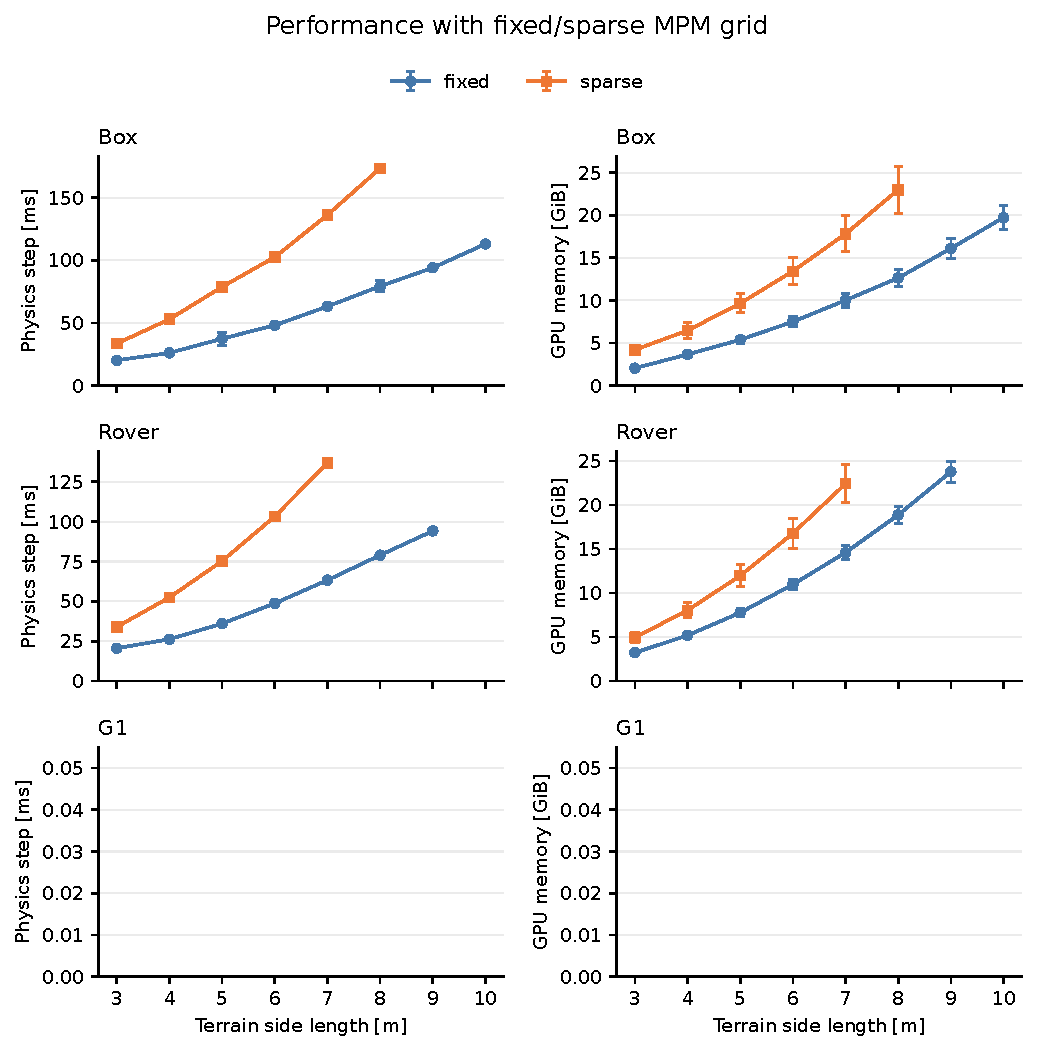
\includegraphics[width=0.88\linewidth]{01_grid_comparison.pdf}
\caption{Fixed and sparse grids using matched initial particle allocations.}
\end{figure}
\begin{figure}[htbp]
\centering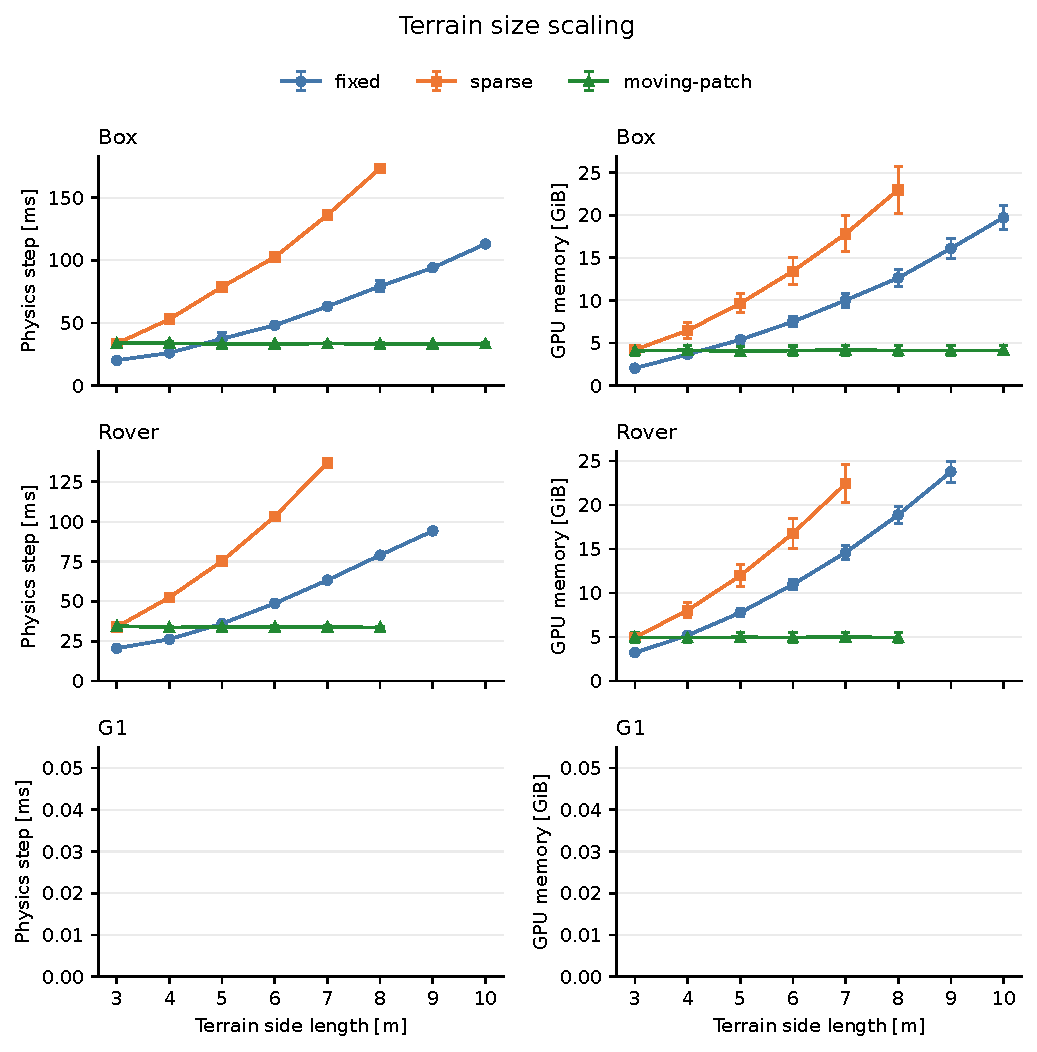
\includegraphics[width=0.88\linewidth]{02_terrain_scaling.pdf}
\caption{Full-terrain methods and the bounded moving particle allocation. Background height samples still grow with terrain extent.}
\end{figure}

For box, fixed changes from 20.15 to 112.93 ms and from 2.04 to 19.72 GiB between 3 and 10 m.

For box, moving-patch changes from 33.70 to 33.37 ms and from 4.09 to 4.13 GiB between 3 and 10 m.

At equal 2 m allocation for box, fixed takes 17.99 ms, sparse 24.01 ms, and moving-patch 24.19 ms. Moving-patch differs from sparse by 0.8 percent.

Moving-patch versus fixed includes both the grid-method difference and patch maintenance. The equal-allocation comparison against sparse more closely measures added patch handling, although material motion can also differ.


\begin{table}[htbp]
\centering\small
\begin{tabular}{lllrrr}
\toprule
Scene & Method & Side [m] & Step [ms] & Steady [GiB] & Peak [GiB] \\
\midrule
box & fixed & 3 & $20.15\pm0.88$ & $2.04\pm0.19$ & 2.56 \\
box & sparse & 3 & $33.52\pm1.04$ & $4.20\pm0.49$ & 4.91 \\
box & moving-patch & 3 & $33.70\pm1.04$ & $4.09\pm0.53$ & 4.91 \\
box & fixed & 10 & $112.93\pm1.14$ & $19.72\pm1.41$ & 20.69 \\
box & moving-patch & 10 & $33.37\pm1.13$ & $4.13\pm0.53$ & 4.88 \\
rover & fixed & 3 & $20.60\pm0.59$ & $3.23\pm0.15$ & 3.45 \\
rover & sparse & 3 & $33.97\pm0.78$ & $4.95\pm0.56$ & 5.82 \\
rover & moving-patch & 3 & $34.54\pm0.74$ & $4.97\pm0.53$ & 5.72 \\

\bottomrule
\end{tabular}
\caption{Endpoint measurements. Step and steady memory show mean $\pm$ standard deviation; peak is the largest sampled value across repeats. Excluded attempts are listed in README.md.}
\end{table}

\section{Equal particle allocation}
The equal-allocation experiment uses particle beds with side lengths 1, 2, and 4 m, with a $0.1\,\mathrm{m}$ boundary on each side for every method. It measures total simulation cost at matched initial allocation, including changes in the physical workload caused by recycling. It does not isolate the cost of individual kernels.
\begin{figure}[htbp]
\centering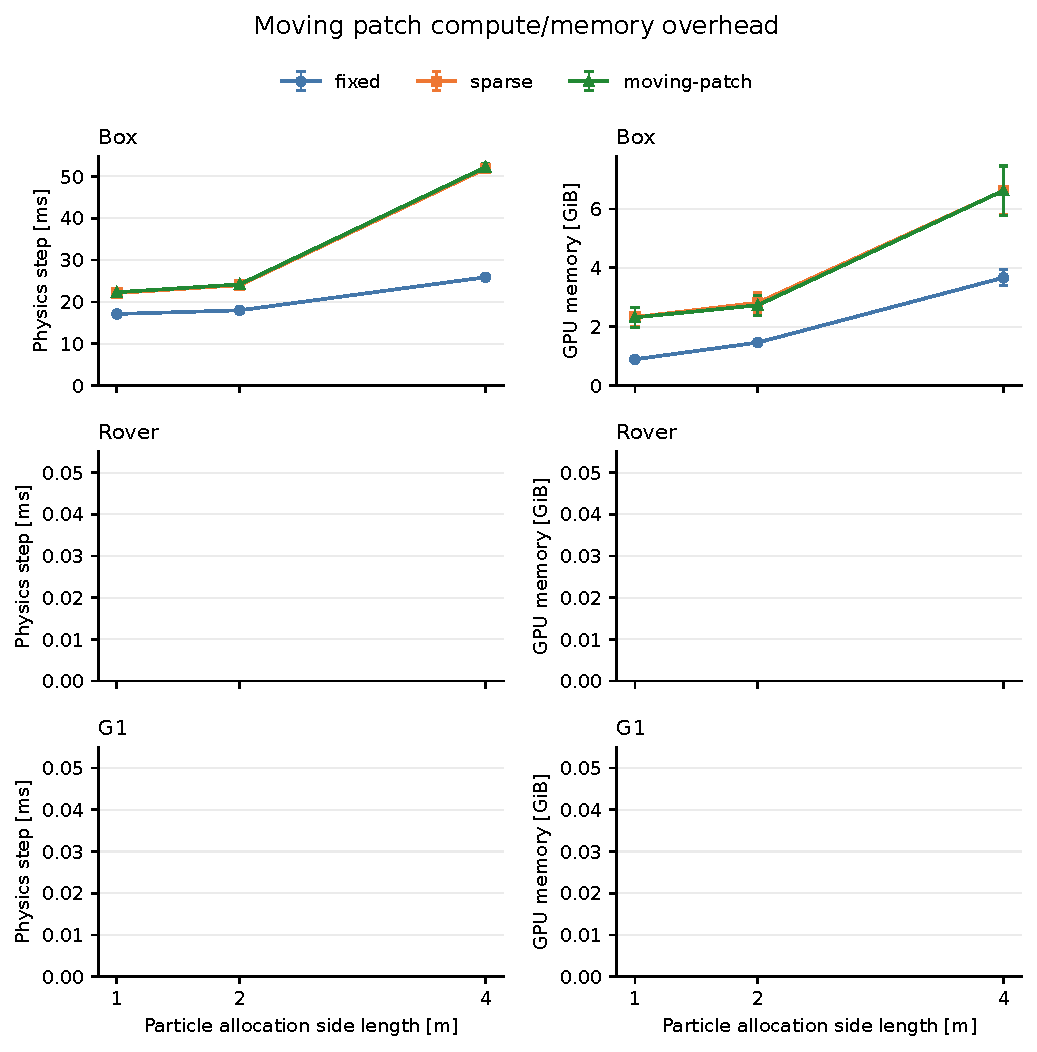
\includegraphics[width=0.88\linewidth]{03_equal_size_comparison.pdf}
\caption{Physics time and GPU memory at matched initial particle counts.}
\end{figure}

\section{Limitations and reproduction}
Short runs may not move far enough to trigger a discrete patch shift. Additional moving-patch cases measure 1200 steps after warm-up, or six simulated seconds, with the default 0.4 m shift interval. Their timings, memory usage, and observed shift counts are reported in README.md.

Alpha includes 31 vertical sampling layers under these settings; beta used 30. Current assets, solver source, and collider handling also differ. These measurements therefore compare methods within alpha and do not establish an alpha-versus-beta speed ratio. A fixed particle allocation bounds MPM particle cost but does not bound storage for all sampled background heights.

Finite-state checks and solver-capacity warnings are recorded. Successful timing runs are not proof of locomotion stability, and the short scaling runs do not traverse the entire terrain. Raw JSON files retain poses, timings, allocation counts, capacities, and memory samples. See README.md for failed attempts, source hashes, asset hashes, and reproduction commands.
\end{document}
